Nim 和: \(a\oplus b:=\operatorname{mex}\left(\{a'\oplus b:a'<a\}\cup\{a\oplus b':b'<b\}\right)\)

Nim 积: \(a\otimes b:=\operatorname{mex}\{(a'\otimes b)\oplus(a\oplus b')\oplus(a'\otimes b'):a'<a,b'<b\}\)

\begin{figure}[h]
    \label{img:nim-add}
    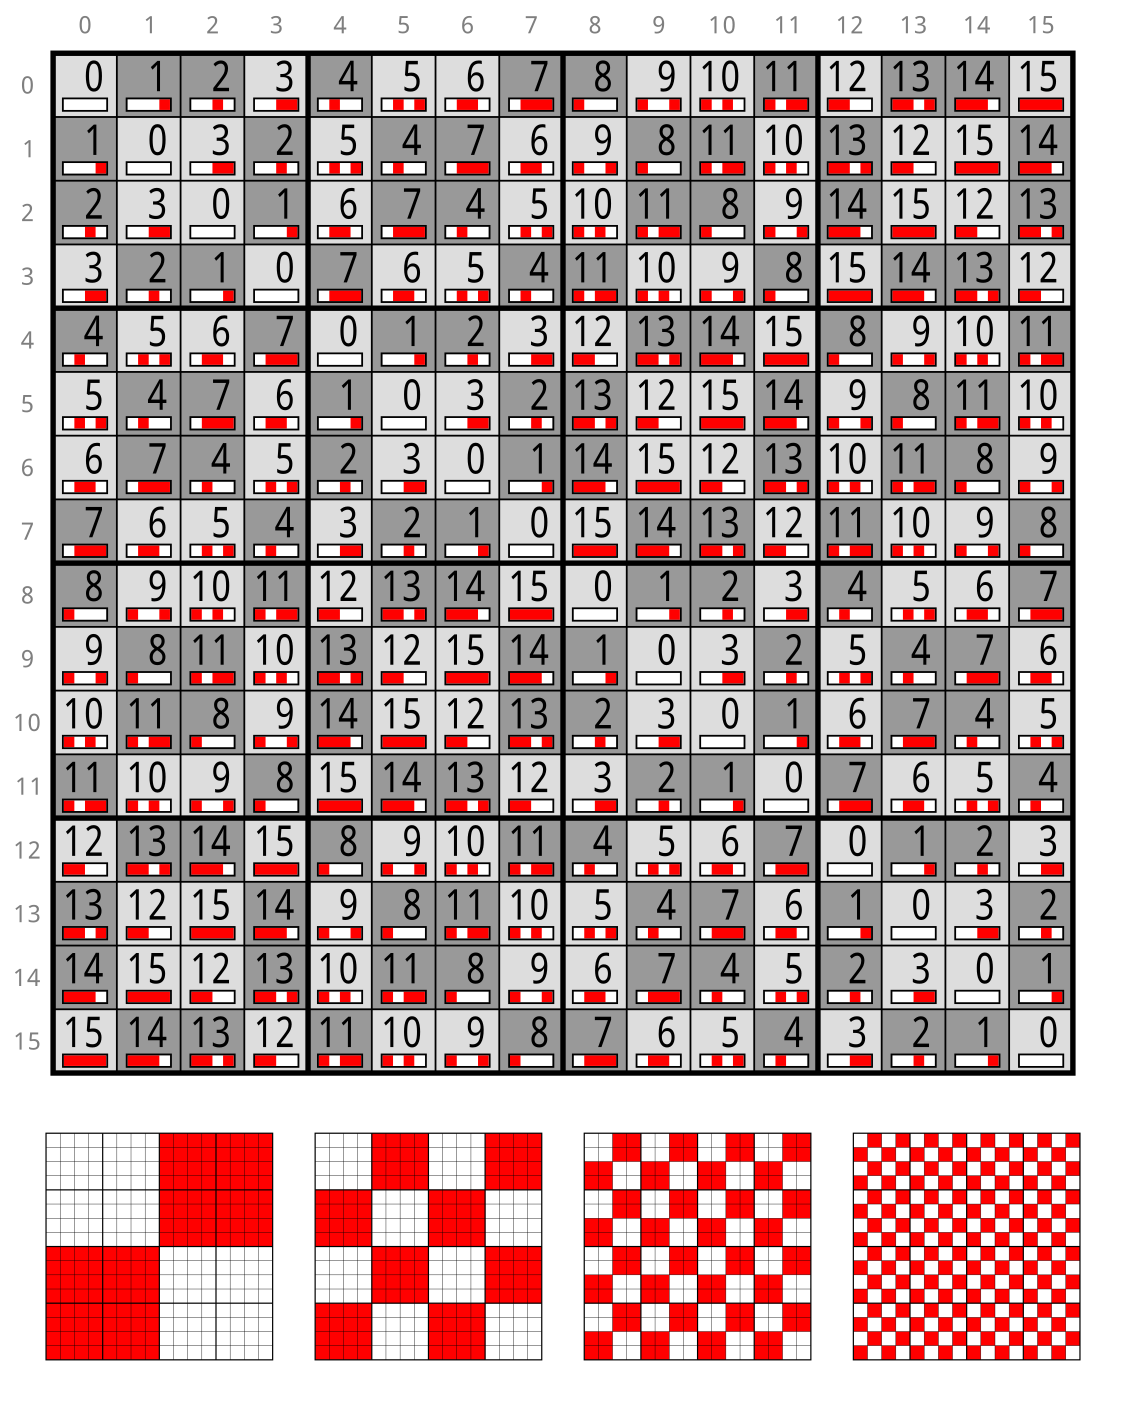
\includegraphics[width=0.7\textwidth]{img/Nimber-addition.svg}
    \caption{Nim 和(From Wikipedia)}
\end{figure}

\begin{figure}[h]
    \label{img:nim-prod}
    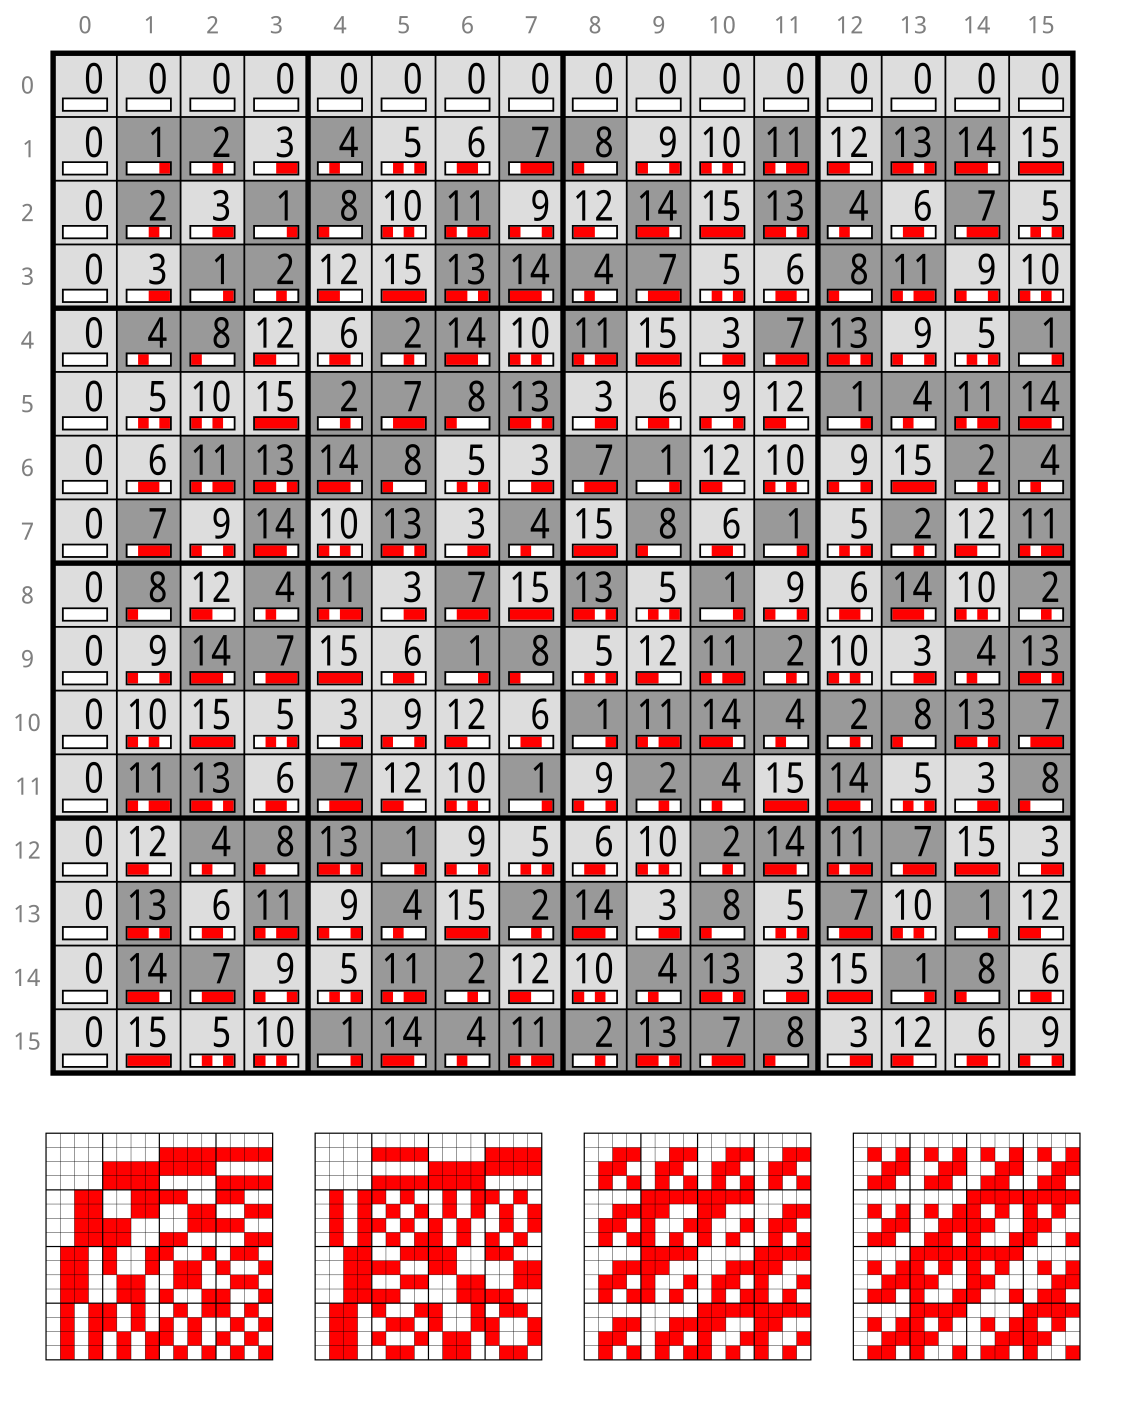
\includegraphics[width=0.7\textwidth]{img/Nimber-multiplication.svg}
    \caption{Nim 积(From Wikipedia)}
\end{figure}

\begin{figure}[h]
    \label{img:nim-prod-pow2}
    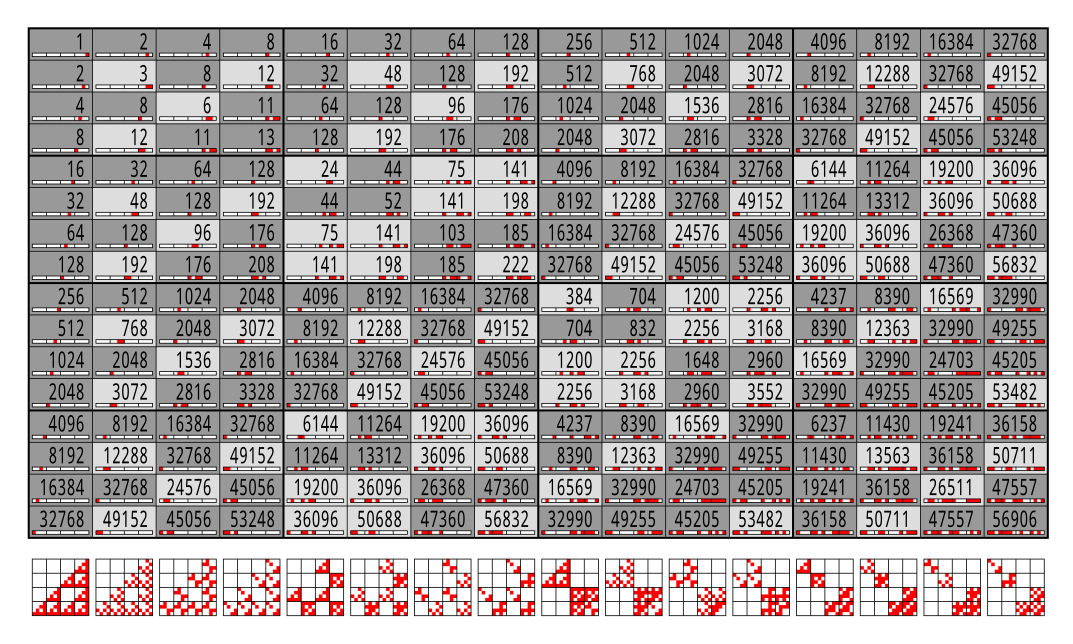
\includegraphics[width=0.7\textwidth]{img/Nimber-multiplication-of-powers-of-two.svg}
    \caption{Nim 积(2 的幂次, From Wikipedia)}
\end{figure}

\paragraph{参考链接}

\url{https://en.wikipedia.org/wiki/Nimber}
